\documentclass[final]{beamer}

\usepackage[scale=1,size=custom,width=106.68,height=83.82,20pt]{beamerposter} % Use the beamerposter package for laying out the poster

\usetheme{confposter} % Use the confposter theme supplied with this template

\setbeamercolor{block title}{fg=ngreen,bg=white} % Colors of the block titles
\setbeamercolor{block body}{fg=black,bg=white} % Colors of the body of blocks
\setbeamercolor{block alerted title}{fg=white,bg=dblue!70} % Colors of the highlighted block titles
\setbeamercolor{block alerted body}{fg=black,bg=dblue!10} % Colors of the body of highlighted blocks
\setbeamertemplate{caption}[numbered]
% Many more colors are available for use in beamerthemeconfposter.sty

%-----------------------------------------------------------
% Define the column widths and overall poster size
% To set effective sepwid, onecolwid and twocolwid values, first choose how many columns you want and how much separation you want between columns
% In this template, the separation width chosen is 0.024 of the paper width and a 4-column layout
% onecolwid should therefore be (1-(# of columns+1)*sepwid)/# of columns e.g. (1-(4+1)*0.024)/4 = 0.22
% Set twocolwid to be (2*onecolwid)+sepwid = 0.464
% Set threecolwid to be (3*onecolwid)+2*sepwid = 0.708

\newlength{\sepwid}
\newlength{\onecolwid}
\newlength{\twocolwid}
\newlength{\threecolwid}
\setlength{\paperwidth}{42in} % 42
\setlength{\paperheight}{33in} % 33
%\setlength{\sepwid}{0.05\paperwidth} % Separation width (white space) between columns
\setlength{\onecolwid}{0.3\paperwidth} % Width of one column
\setlength{\topmargin}{-0.5in} % Reduce the top margin size
%-----------------------------------------------------------

\usepackage{tikz}
\usepackage{lipsum}
\usepackage{graphicx}  % Required for including images
\usepackage{siunitx}
\usepackage{booktabs} % Top and bottom rules for tables
\usepackage{subcaption}
\usepackage{wrapfig}


\newcommand{\pder}[2]{\frac{\partial#1}{\partial#2}}
\newcommand{\pdder}[2]{\frac{\partial^2#1}{\partial#2^2}}
\newcommand{\myabs}[1]{\vert#1\vert}

\DeclareMathOperator{\iso}{Iso}
\DeclareMathOperator{\fix}{Fix}
\DeclareMathOperator{\tr}{Tr}
%-----------------------------------------------------------
%	TITLE SECTION 
%-----------------------------------------------------------

\title{Hearing the Local Orientability of Orbifolds} % Poster title

\author{Sean Richardson '20, Liz Stanhope} % Author(s)

\institute{Department of Mathematical Sciences, Lewis \& Clark College} % Institution(s)

\begin{document}

\addtobeamertemplate{block end}{}{\vspace*{2ex}} % White space under blocks
\addtobeamertemplate{block alerted end}{}{\vspace*{2ex}} % White space under highlighted (alert) blocks

\setlength{\belowcaptionskip}{2ex} % White space under figures
\setlength\belowdisplayshortskip{2ex} % White space under equations

\begin{frame}[t] % The whole poster is enclosed in one beamer frame
\begin{columns}[t] % The whole poster consists of three major columns, the second of which is split into two columns twice - the [t] option aligns each column's content to the top

%--------------------------------------------------------
%   CONTENT
%-------------------------------------------------------- 


%---------------------------------------------------------
%   COLUMN 1
% --------------------------------------------------------
\begin{column}{\onecolwid} % The first column

% --------------------------------------------------------
%   SYMMETRIES OF SPACE
% --------------------------------------------------------
    \begin{block}{Symmetries of Space}
    A pattern with symmetry has a group of actions $\Gamma$ we can perform
    on the pattern without change. For instance, we can rotate
    Figure~\ref{fig:rot_sym} by any element of $\Gamma  = \{\ang{0}, \ang{90}, \ang{180}, \ang{270}\}$
    and still preserve the pattern. Similarly, Figure~\ref{fig:ref_sym} is
    preserved by doing nothing and reflecting along the diagonal. Notice
    these actions do not alter the size of the patterns, making them
    \emph{isometries}.
    \begin{figure}[c]
        \begin{subfigure}[c]{0.25\textwidth}
        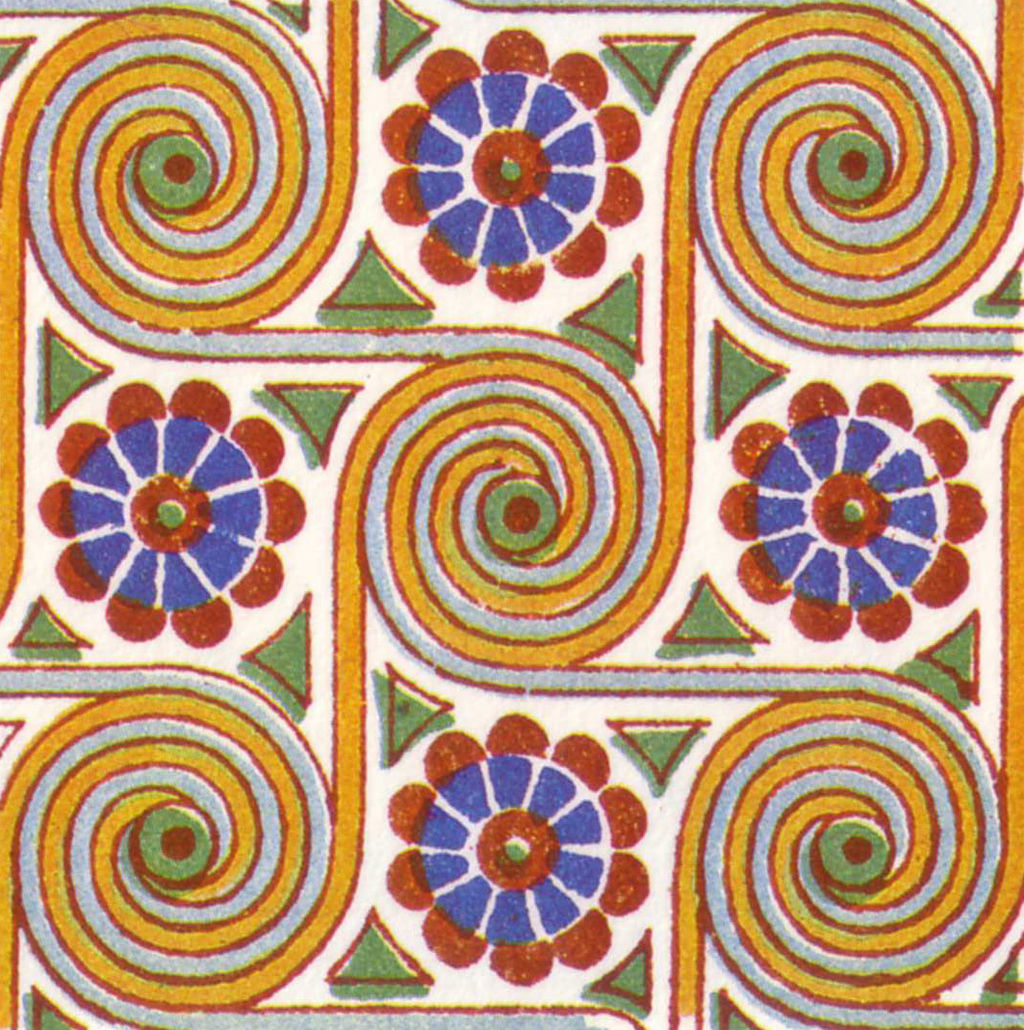
\includegraphics[width=\textwidth]{images/p4_symmetry_wallpaper.jpg}
        \caption{Rotational Symmetry}
        \label{fig:rot_sym}
        \end{subfigure}
        \begin{subfigure}[c]{0.2\textwidth}
            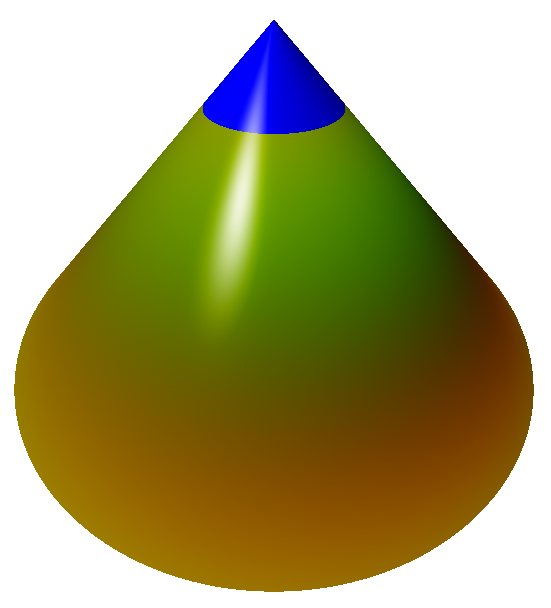
\includegraphics[width=\textwidth]{images/cone_point.png}
            \caption{Cone Point}
        \end{subfigure}
        \begin{subfigure}[c]{0.25\textwidth}
        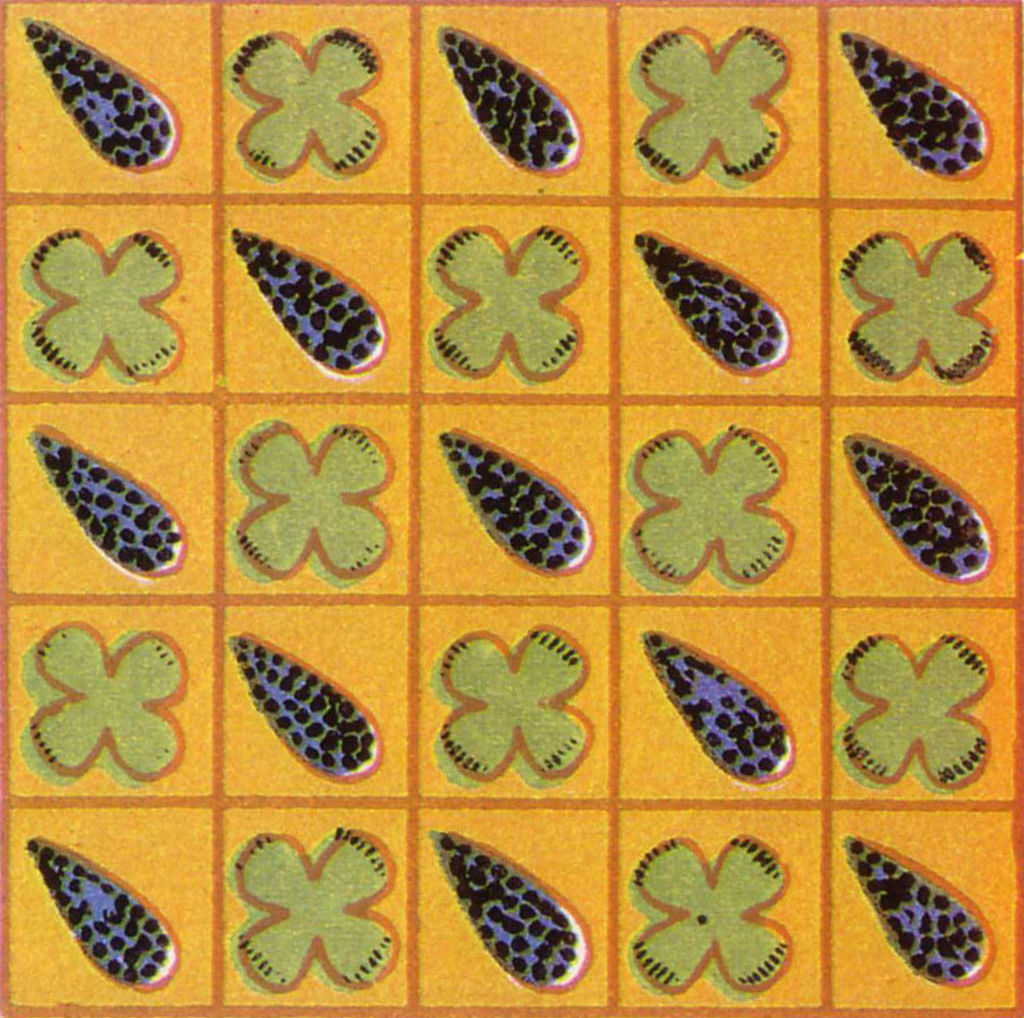
\includegraphics[width=\textwidth]{images/reflection_symmetry_wallpaper.jpg}
        \caption{Reflectional Symmetry}
        \label{fig:ref_sym}
        \end{subfigure}
        \begin{subfigure}[c]{0.2\textwidth}
            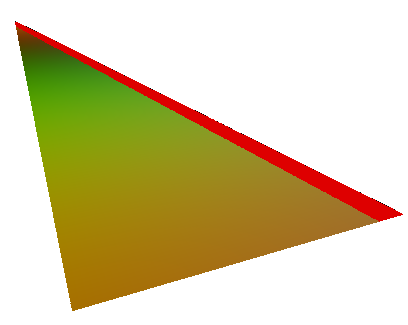
\includegraphics[width=\textwidth]{images/mirror_edge.png}
            \caption{Mirror Edge}
        \end{subfigure}
        \caption{Folding Symmetries}
        \label{fig:sym}
    \end{figure}

    To visualize symmetry we imagine folding patterns on pieces of paper
such that each piece of the pattern occurs only once. In
Figure~\ref{fig:ref_sym}, we can fold the pattern across the diagonal,
creating half plane with a sharp edge. In Figure~\ref{fig:rot_sym}, we can
roll up the pattern into a party hat shape, creating a sharp point. We
denote these resulting shapes $\mathbb{R}^n/\Gamma$ where $\Gamma$ is the
symmetry group of the pattern. The sharp parts of the shapes are \emph{strata}. 

\end{block}

% --------------------------------------------------------
%   ORBIFOLDS
% --------------------------------------------------------

\begin{block}{Orbifolds}
        \begin{columns}[t]
        \begin{column}[t]{0.55\textwidth}
An orbifold is a generalization of a simple $n$ dimensional surface, which we
call a manifold. If you were to zoom into a manifold, you
will see flat space, for it has local structure $\mathbb{R}^n$. However, an
orbifold allows local structure of $\mathbb{R}^n/\Gamma$ (such as the
cone point or mirror edge in Figure~\ref{fig:sym}). Figure~\ref{fig:orb_ex}
is a visual representation of a two dimensional orbifold with a cone point and a mirror
edge.
        \end{column} 
        \begin{column}[t]{0.45\textwidth}
        \begin{figure}
        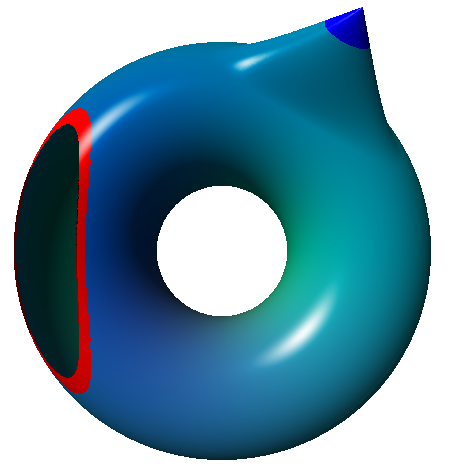
\includegraphics[width=0.7\textwidth]{images/orbifold_ex.png}
        \caption{Orbifold Representation}
        \label{fig:orb_ex}
        \end{figure}
        \end{column}
        \end{columns}
    \end{block}
%--------------------------------------------------------- 
%   LAPLACE SPECTRA
%--------------------------------------------------------- 

    \begin{block}{Laplace Spectra}
A string on the guitar produces a sound determined by a specific frequency
it can vibrate at. Actually, the string can vibrate at a \emph{spectrum} of
resonance frequencies. All objects have such a vibrational spectrum ---
drums will vibrate at only certain sounds. Mathematically, we express these
frequencies through the \emph{Laplace Spectra}.

The Laplace Spectra follows from the wave equation, $\Delta u =
\pdder{u}{t}$, which describes the amplitude $u(t,\mathbf{x})$ at any location
$\mathbf{x}$ and time $t$ on an orbifold. In assuming
$u(t,\mathbf{x})=A(t)\psi(x)$ for standing wave solutions, we find $\Delta u
= -\lambda \psi(\mathbf{x})$. The eigenvalue solutions
$\lambda_1,\lambda_2,\dots$ are called the Laplace Spectra where each
$\sqrt{\lambda_i}$ is a valid fundamental frequency.
    \end{block}

\end{column}
\begin{column}{\onecolwid} % The 2nd column
\begin{block}{Research Question}

Given a specific drum, it is possible to deduce what sound the drum will
make when hit. However, consider the reverse: if you hear a drum in the
neighboring room, is it possible to reverse engineer the drum's shape? In other words, ``can you hear
the shape of a drum?'' In this research we ask a similar question: Can you
hear the shape of an orbifold?

Formally, consider some Laplace Spectra $\lambda_1, \lambda_2, \dots$
belonging to some unknown orbifold $\mathcal{O}$. From the Laplace Spectra,
what properties can we deduce about $\mathcal{O}$?

\end{block}

\begin{block}{Local Orientability}
Isometries can preserve or reverse orientation. For instance, a reflection
reverses orientation (when you look into a mirror, your reflection is
flipped), but a simple rotation preserves orientation. 

Some local structure of an orbifold $\mathbb{R}^n/\Gamma$ has a group of 
isometries $\Gamma$ associated with it. If $\Gamma$ contains a single
orientation reversing isometry, the local structure is
\emph{non-orientable}; otherwise, it is \emph{orientable}.

We define an orbifold to be \emph{locally non-orientable} if it has a
single non-orientable local structure; otherwise, the orbifold is
\emph{locally orientable}.

\end{block}

\begin{block}{Result}
    \begin{columns}[t]
        \begin{column}[t]{0.4\textwidth}
    We found you can hear the local orientability of an orbifold ---
    there exists no locally orientable orbifold and locally non-orientable orbifold
    with the same Laplace Spectra. Figure~\ref{fig:result_ex} shows two
    orbifolds guaranteed to have different Laplace Spectra by this result.
    \end{column}
    \begin{column}[t]{0.59\textwidth}
        \begin{figure}
        \begin{subfigure}[t]{0.49\textwidth}
            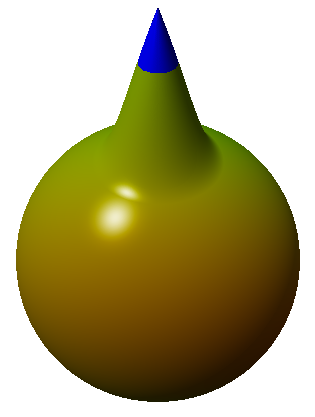
\includegraphics[width=\textwidth]{images/teardrop.png} 
        \end{subfigure}
        \begin{subfigure}[t]{0.49\textwidth}
            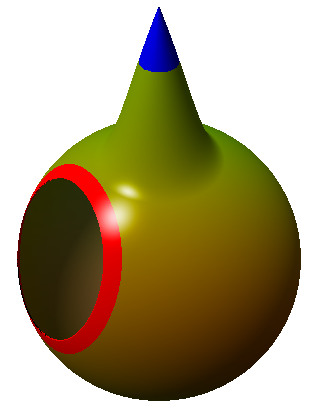
\includegraphics[width=\textwidth]{images/teardrop_edge.png}
        \end{subfigure}
        \caption{Non-isospectral Orbifolds}
        \label{fig:result_ex}
    \end{figure}
    \end{column}
    \end{columns}
\end{block}
\begin{block}{Future Work}
\begin{columns}[t]
    \begin{column}[t]{0.61\textwidth}
In addition to this result, we studied symmetry patterns of $3$
dimensional space, which are called the crystallographic space groups. Each space group
of isometries can be folded into a $3$ dimensional orbifold (visualized in
higher dimensional space). These orbifolds have a Laplace Spectra we can
study. There are $230$ such patterns and corresponding orbifolds, so perhaps
a computer can automate the process of finding heat expansion coefficients.
\end{column}
\begin{column}[t]{0.37\textwidth}
\begin{figure}
    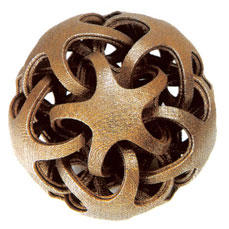
\includegraphics[width=\textwidth]{images/space_group_sym.jpg}
    \caption{Spacial Symmetry from \textit{The Symmetries of Things}}
\end{figure}
\end{column}
\end{columns}
\end{block}
\end{column}
\begin{column}{\onecolwid} % The 3rd column
    \begin{block}{Asymptotic Heat Expansion}
        Our question requires us to relate the properties of the orbifold
        to its Laplace Spectra, which can be done by studying how heat
        disperses throughout the orbifold. This section will touch on the
        logic used to prove our result.
        
        Consider focusing heat at a single point $\mathbf{x}$ on some
        orbifold $\mathcal{O}$.  Then, allow the heat to disperse around
        $\mathcal{O}$. The point $\mathbf{x}$ will cool with
        time. We study a specific function: how a point cools on average for
        every point in $\mathcal{O}$, which is known to be
        $\sum_{i=1}^{\infty}e^{-\lambda_i t}$ where $\lambda_i$ is an
        element of the Laplace Spectrum of $\mathcal{O}$. Formally, this
        falls out of the heat equation, $\Delta u = \pder{u}{t}$. The
        integrand of the solution is the heat kernel $K$, and we find that
        $\tr(K) = \sum_{i=1}^{\infty}e^{-\lambda_i t}$.
        
        If we approximate this function for small values of time, we get a
        function of the following form (for $2$ dimensions)

        \begin{equation*}
            \sum_{i=1}^{\infty}e^{-\lambda_i t} \sim
            \frac{a}{t}+\frac{b}{\sqrt{t}}+c+d\sqrt{t}+\dots
        \end{equation*}
        Where the right side approximates the left for small $t$ as in
        Figure~\ref{fig:asym_aprox}.
   
        \begin{columns}[t]
        \begin{column}[c]{0.43\textwidth}
        \begin{figure}
        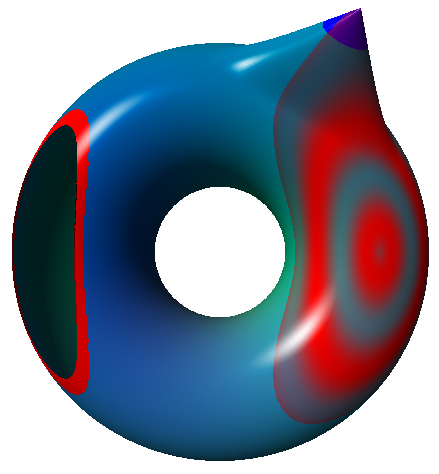
\includegraphics[width=\textwidth]{images/heat_ex.png}
        \caption{Heat dispersing from $\mathbf{x}$}
        \label{fig:heat_ex}
        \end{figure}
        \end{column}
        \begin{column}[c]{0.55\textwidth}
        \begin{figure}
        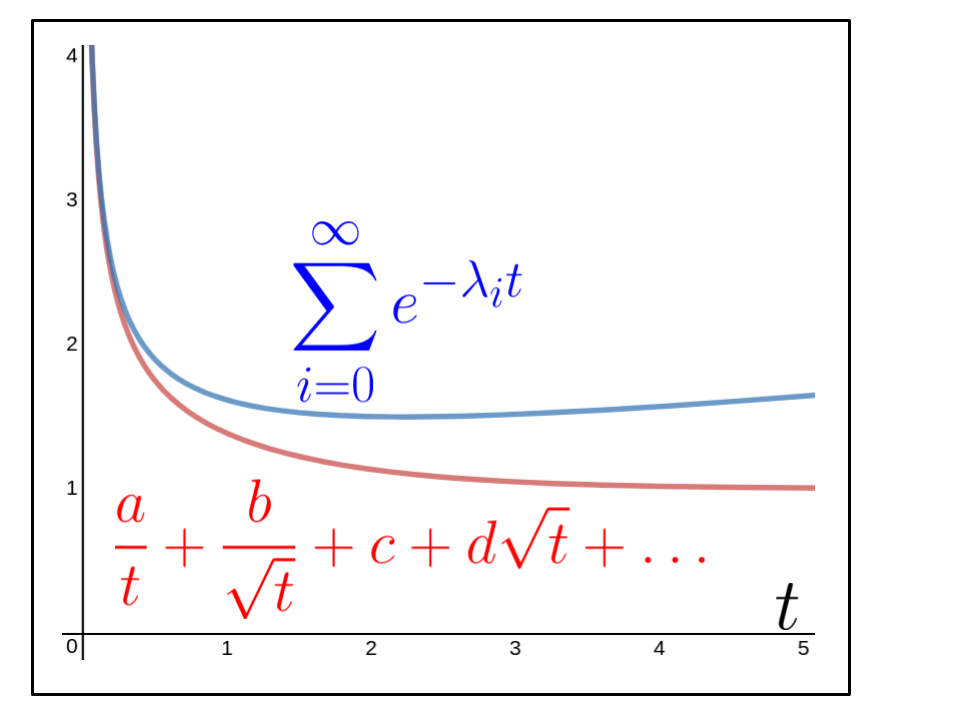
\includegraphics[width=\textwidth]{images/heat_exp_graph2.png}
        \caption{Asymptotic Expansion Approximation}
        \label{fig:asym_aprox}
        \end{figure}
        \end{column}
        \end{columns}
        The resulting equation has coefficients $a,b,c,\dots$. We can find
        these coefficients from the properties of $\mathcal{O}$. The
        coefficients are described by
        
       \begin{align*}
           &{(4\pi t)}^{-\dim(\mathcal{O})/2}\sum_{k=0}^{\infty}a_k(\mathcal{O})t^k \\
            &+\sum_{N \in S(\mathcal{O})}\frac{{(4\pi t)}^{-\dim(N)/2}}{\myabs{\iso(N)}}\sum_{k=0}^{\infty}t^k\int_{N} \sum_{\gamma \in \iso^{\max}(\tilde{N})}b_k(\gamma,x) dvol_N
       \end{align*}
        
        So, properties of $\mathcal{O}$ determine coefficients
        $a,b,c,\dots$ and the coefficients determine the Laplace Spectra
        $\lambda_1,\lambda_2,\dots$. If two orbifolds differ in a
        single coefficient, they will have different Laplace Spectra.  In
        our proof, we use the fact that in odd dimensions, only isometries
        with even dimensional strata are orientation reversing (and vice
        versa for even dimensions). With this, we show that the
        locally orientable and locally non-orientable orbifolds are
        guaranteed to differ in at least one coefficient, implying different
        Laplace Spectra.

    \end{block}
    
    \begin{block}{\normalsize{Acknowledgments}}
    Many thanks to the John S. Rogers Science Program and James F. and Marion L. Miller Foundation for funding this research. 
    \textit{Asymptotic Expansion of the Heat Kernel for
    Orbifolds} provided many results used in our proof.
    \end{block}

    \end{column}
\end{columns}
\end{frame}
\end{document}
